% Pacotes
\documentclass[12pt]{article}
\usepackage{adjustbox}
\usepackage[utf8]{inputenc}
\usepackage{amsmath}
\usepackage{hyperref}
\usepackage{sbc-template}
\usepackage{fancyvrb}
\usepackage{amsfonts}
\usepackage{amsmath}
\usepackage{graphicx,url}


\sloppy

\title{Atom\\O Editor Open Source do GitHub}

\author{Ricardo Henrique Brunetto\inst{1}}


\address{Departamento de Informática -- Universidade Estadual de Maringá (UEM)\\
	Maringá -- PR -- Brasil
	\email{ra94182@uem.br}
}

\begin{document}

	\maketitle

	{\resumo{O presente trabalho visa a apresentar de forma instrutiva as funcionalidades do editor de texto Atom e tratar a respeito de suas vantagens, desvantagens, formas de instalação e recursos que o diferenciam dos demais editores. Este trabalho segue referência direta da documentação oficial do Atom \cite{doc:atom}, embora algumas seções não sejam mencionadas a fim de manter concisão.}}

	\newpage
	\tableofcontents
	\newpage

  \section{Introdução}\label{sec:intro}
	O Atom é um editor de texto de código aberto desenvolvido pelo GitHub e liberado como beta em junho de 2015, projetado para combinar flexibilidade e extensibilidade. De forma geral, o Atom é um editor focado em desenvolvimento de código, oferecendo recursos e ferramentas para solucionar dos mais ínfimos aos mais significativos inconvenientes do ofício. Além disso, por ser um software livre e aberto e fornecer suporte à extensões criadas pelos própriros usuários, o Atom passou a ser conhecido como "Editor de Texto Hackeável do Século 21".

	O Atom foi desenvolvido através do Electron e de outras tecnologias web (HTML, Javascript e CSS). O ponto-chave do Atom como editor de texto é um compromisso com a hackeabilidade e usabilidade, o que significa que os principais avanços e diferenciais do software se concentram em proporcionar ao usuário uma forma de personalizar por completo sua experiência. Dessa forma, o usuário consegue criar \textit{plug-ins} e extensões conforme sua necessidade e propósito.

	Dessa forma, o Atom é composto por seu núcleo, ferramentas e componentes que são adotados como oficiais e vêm instalados (bem como o próprio editor), e pelos \textit{add-ons} desenvolvidos pelos próprios usuários e disponíveis em repositórios na web (em especial no GitHub). A respeito do núcleo do Atom, alguns aspectos são interessantes e passíveis de abordagem.

	Duas décadas de desenvolvimento Web permitiram que a mesma evoluísse para uma incrível e poderosa plataforma. Contudo, codificar é uma tarefa especial que requer ferramentas dedicadas. Por isso, o Atom não foi escrito como uma aplicação web tradicional, mas sim como uma variante específica do Chromium, dedicada à escrita de texto.

	Abrindo um rápido parênteses, o Chromium é um conjunto de projetos que incluem um navegador web de código aberto e livre que a Google usa como base para o desenvolvimento do Google Chrome, e um sistema operacional onde a Google também se baseia para o Chrome OS. Mais informações podem ser encontradas em \cite{doc:chromium}.

	Outro grande benefício é garantir que tudo está rodando na mais nova versão do Chromium. Isso significa que não há preocupações em relação à compatibilidade ou versionamentos. Dessa forma, os mais recentes recursos e frameworks desenvolvidos na Web para uso em aplicações podem ser incluídos no Atom sem que haja problemas de compatibilidade com projetos já em desenvolvimento.

	Desenvolver um editor de texto baseado em tecnologias Web é um acerto no sentido em que se tem grande capacidade de crescimento, visto que, embora as tecnolgias nativas variem entre si, as tecnologias Web permanecem por serem multi-plataforma e irrestritas quanto às possiblidades de desenvolvimento.

	De acordo com os próprios desenvolvedores, o Atom exerce um papel complementar à função do GitHub de proporcionar software melhor através do trabalho em equipe, o que implica que o editor é, na verdade, um investimento à longo prazo, sempre respaldado pelo suporte do próprio GitHub. Além disso, conforme outros editores como Emacs e Vim demonstraram com o passar dos anos, o desenvolvimento de um software estável, de grande comunidade e eficiente, necessita ter código aberto.

	\section{Instalação}

	Disponível nos sitemas operacionais Mac, Windows e Linux, instalar o Atom é realmente simples, em todos eles. O primeiro passo é fazer o \textit{download} da versão compatível com o sistema operacional em \href{https://atom.io}{https://atom.io}.

	A seguir serão explorados detalhes particulares da instação do Atom em cada um dos sistemas operacionais em que está disponível.

	\subsection{Instalação no Windows}\label{sec:instwin}
	Dentre as opções de \textit{download} mencionadas acima, há uma versão com o \textit{Windows Installer}. Após realizar a instalação seguindo as instruções do instalador, será instalado o Atom,bem como seus atalhos na área de trabalho e menu de inicialização, e serão adicionados os comandos \verb|atom| e \verb|apm| na variável do sistema \verb|PATH|, para que também se possa manipular o programa por linha de comando através do terminal (no Windows, \verb|cmd|).

	Além disso, as opções \verb|Abrir com Atom| e as associações em \verb|Abrir com...| serão criadas automaticamente. Contudo, isso pode ser controlado através de um painel no próprio Atom. Basta acessar o menu \verb|File > Settings| e escolher \verb|System| no painel lateral. Em ordem, de acordo com a Figura \ref{fig:fig1}, as opções: Registra o Atom no menu de associação de arquivos (\verb|Abrir com...|); Mostra a opção \verb|Abrir com Atom| no menu de contexto de arquivos; Mostra a opção \verb|Abrir com Atom| no menu superior do Explorer.

	\begin{figure}[h]
		\centering
		\label{fig:fig1}
		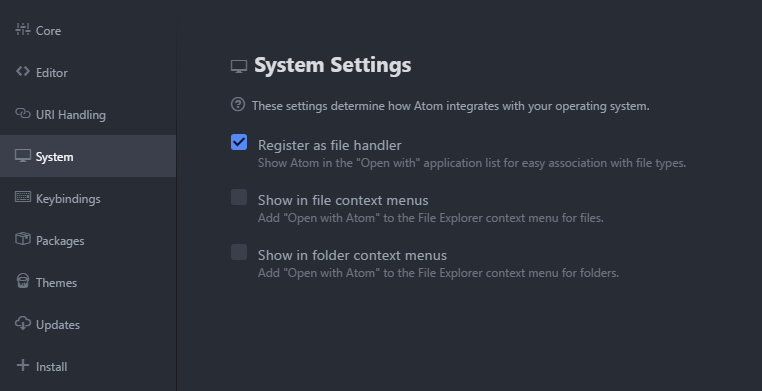
\includegraphics[scale = 0.7]{fig1}
		\caption{Menu de controle das opções do Sistema no Windows.}
	\end{figure}

	\subsubsection{Modo Portátil}\label{sec:portable}
	O Atom possui um Modo Portátil (\textit{Portable Mode}) disponível para ser utilizado.

	As configurações e estados do Atom são armazenados em \textit{\%userprofile\%$\backslash$.atom} (no Windows, \textit{\%userprofile\%} por padãro referencia \textit{C:$\backslash$users$\backslash$NOME\_DE\_USUARIO}). Assim, o usuário pode executar o Atom com modo portátil onde o programa e suas configurações estão armazenados juntos, tal como em um dispositivo de armazenamento removível (\textit{ex: pendrives}).

	Para configurar o modo portátil, basta fazer o download da versão correspondente ao sistema operacional em \href{https://github.com/atom/atom/releases/latest}{https://github.com/atom/atom/releases/latest} e extrair no dispositivo de armazenamento removível. Após isso, crie uma pasta intitulada \textit{.atom} no mesmo diretório que contém a pasta extraída. Por exemplo, se a extração foi realizada em \textit{E:$\backslash$}, então deve-se ter:
	\begin{Verbatim}[fontsize=\footnotesize]
		E:\atom-1.14\atom.exe
		E:\.atom
	\end{Verbatim}
	Algumas observações em relação ao Modo Portátil são válidas:
	\begin{enumerate}
		\item O diretório \textit{.atom} deve ser gravável (\textit{writable});
		\item Não é necessário criar a pasta \textit{.atom}. Pode-se copiar uma já existente;
		\item O Atom pode armazenar configurações de usuário do Electron na pasta \textit{electronUserData};
		\item Tambem é possível criar uma variável de ambiente \verb|ATOM_HOME| para referenciar o diretório \textit{.atom} ou um script (\textit{.sh, .cmd}) para inicializá-lo;
		\item A instação em Modo Portátil \textbf{não} atualizará automaticamente.
	\end{enumerate}

	\subsubsection{Configurações de Firewall e Proxy}\label{sec:fireproxy}
	Em caso de problemas com o Firewall ou erros de SSL ao instalar os pacotes, pode-se desativar a opção de rigorosidade do SSL através do prompt de comando do (no Windows: \verb|[Win + R] > cmd > [ENTER]|) com a seguinte linha de comando:
	\begin{Verbatim}[fontsize=\footnotesize]
		apm config set strict-ssl false
	\end{Verbatim}

	Caso o problema seja em relação ao Proxy, pode-se configurar um proxy HTTP(S) através da seguinte linha de comando:
	\begin{Verbatim}[fontsize=\footnotesize]
		apm config set https-proxy SEU_ENDERECO_PROXY
	\end{Verbatim}
	onde \verb|SEU_ENDERECO_PROXY| é o endereço de proxy a ser utilizado.

	\subsection{Mac}
	De forma semelhante à instalação no Windows (vide Seção \ref{sec:instwin}), a instação do Atom segue o padrão do sistema operacional. Nesse caso, o padrão zip para as instalações no Mac. O \textit{download} pode ser feito alternativamente em \href{https://github.com/atom/atom/releases/latest}{https://github.com/atom/atom/releases/latest} através do arquivo \textit{atom-mac.zip}. Após baixar o arquivo, basta extraí-lo e arrastar o \verb|Atom| para a pasta \textit{Aplicações} (ou \textit{Applications}).

	Ao abrir a aplicação pela primeira vez, os comandos \verb|atom| e \verb|apm| serão instalados. Em alguns casos, o Atom pode não conseguir realizar esta etapa, visto que pode ser necessária a senha do adminstrador. Para verificar se houove sucesso, basta abrir o terminal de comando do Mac e inserir a linha de comando \verb|which atom|. Em caso de sucesso, será retornado o local de instalação (em geral, \verb|/usr/local/bin/atom|) e, caso contrário, nada será retornado.

	Uma nova tentativa de instalação dos comandos pode ser feita na Paleta de Comandos (\textit{Command Palette}) do Atom (explanada na Seção \ref{sec:commandpalette}) através do seguinte comando: \verb|Window: Install Shell Commands|.

	\subsubsection{Modo Portátil}
	As configurações de instalação e as observações válidas são exatamente como mencionado na Seção \ref{sec:portable}. As diferenças, contudo, estão na forma como os arquivos são organizados. No Mac, a hierarquia das pastas para a configuração do modo portátil (\textit{.atom}) seria:
	\begin{Verbatim}[fontsize=\footnotesize]
		/MyUSB/Atom.app
		/MyUSB/.atom
	\end{Verbatim}

	Além disso, as configurações e estados do Atom \textbf{não} são armazenados em \textit{\%userprofile\%$\backslash$.atom} pois o Mac não fornece uma variável \textit{\%userprofile\%}, sendo tais configurações armazenadas na pasta \textit{home} do usuário.

	\subsubsection{Configurações de Firewall e Proxy}
	Em caso de problemas com Firewall ou Proxy, basta seguir as instruções da Seção	\ref{sec:fireproxy}, pois os comandos (e suas sintaxes) são idênticos nos sistemas operacionais disponíveis.

	\subsection{Linux}
	No Linux, pode-se utilizar o Gerenciador de Pacotes (\textit{Package Manager}) para configurar um dos repositórios oficiais do Atom, o que também permtirá atualizar o Atom quando possível.

	A seguir, serão explanados detalhes para as principais distribuições do Linux onde o Atom está presente. Vale salientar que, para distribuições baseadas nas apresentadas, pode-se seguir as mesmas instruções. \textbf{Todas} as instruções a seguir são realizadas em linha de comando do \textbf{Terminal} do Linux. Não é utilizado o recurso gráfico dos sistemas operacionais para tal. Além disso, todos os comandos que incluirem \verb|sudo| podem requerer senha de administrador.

	\subsubsection{Debian e Ubuntu (deb/apt)}
	Inicialmente, adicionam-se os repositórios oficiais para o Gerenciador de Pacotes das distribuições através das seguintes linhas de comando:
	\begin{Verbatim}[fontsize=\footnotesize]
$ curl -L https://packagecloud.io/AtomEditor/atom/gpgkey | sudo apt-key add -
$ sudo sh -c 'echo "deb [arch=amd64] \
	https://packagecloud.io/AtomEditor/atom/any/ any main" > \
	/etc/apt/sources.list.d/atom.list'
$ sudo apt-get update
	\end{Verbatim}

	Após atualizar os repositórios, instala-se o Atom através do comando \verb|apt-get|:
	\begin{Verbatim}[fontsize=\footnotesize]
$ sudo apt-get install atom
	\end{Verbatim}
	Ou, para instalar o Atom versão Beta:
	\begin{Verbatim}[fontsize=\footnotesize]
$ sudo apt-get install atom-beta
	\end{Verbatim}

	Alternativamente, pode-se instalar o Atom através do pacote \textit{.deb}:
	\begin{Verbatim}[fontsize=\footnotesize]
$ sudo dpkg -i atom-amd64.deb
$ sudo apt-get -f install
	\end{Verbatim}
	onde a segunda linha serve para instalar as dependências do Atom, caso estejam faltando.

	\subsubsection{Red Hat e CentOS ou Fedora}
	Aqui ocorrem dois casos diferentes, uma vez que as distribuições Red Hat e CentOS (e suas derivadas) fazem uso do comando \verb|yum| para instalações, em face ao comando \verb|dnf| usado pelo Fedora e suas derivações.

	Partindo do mesmo princípio, adicionam-se inicialmente os repositórios oficiais do Atom no Gerenciador de Pacotes:
	\begin{Verbatim}[fontsize=\footnotesize]
$ sudo rpm --import https://packagecloud.io/AtomEditor/atom/gpgkey
$ sudo sh -c 'echo -e "[Atom]\nname=Atom \
  Editor\nbaseurl=https://packagecloud.io/AtomEditor/atom/el/7/ \
  \$basearch\nenabled=1\ngpgcheck=0\nrepo_gpgcheck=1 \
  \ngpgkey=https://packagecloud.io/AtomEditor/atom/gpgkey" > \
  /etc/yum.repos.d/atom.repo'
	\end{Verbatim}

	Neste momento, instala-se o Atom através da linha de comando:
	\begin{itemize}
		\item Red Hat / CentOS
		\begin{Verbatim}[fontsize=\footnotesize]
	$ sudo yum install atom
	$ sudo yum install atom-beta
		\end{Verbatim}
		\item Fedora
		\begin{Verbatim}[fontsize=\footnotesize]
	$ sudo dnf install atom
	$ sudo dnf install atom-beta
		\end{Verbatim}
	\end{itemize}

	\subsubsection{Modo Portátil}
	As configurações de instalação e as observações válidas são exatamente como mencionado na Seção \ref{sec:portable}. As diferenças, contudo, estão na forma como os arquivos são organizados. No Linux, a hierarquia das pastas para a configuração do modo portátil (\textit{.atom}) seria:
	\begin{Verbatim}[fontsize=\footnotesize]
		/media/myusb/atom-1.14/atom
		/media/myusb/.atom
	\end{Verbatim}

	Além disso, as configurações e estados do Atom \textbf{não} são armazenados em \textit{\%userprofile\%$\backslash$.atom} pois as distribuições do Linux não fornecem uma variável \textit{\%userprofile\%}, sendo tais configurações armazenadas na pasta \textit{home} do usuário.

	\subsubsection{Configurações de Firewall e Proxy}
	Em caso de problemas com Firewall ou Proxy, basta seguir as instruções da Seção	\ref{sec:fireproxy}, pois os comandos (e suas sintaxes) são idênticos nos sistemas operacionais disponíveis.

	\subsection{Construindo do Código-Fonte}
	Além de baixar o instalador, também é possível compilar diretamente o código-fonte nos sistemas operacionais Mac, Windows, Linux e FreeBSD.

	Os detalhes de como fazer isso estão disponíveis na Seção \ref{sec:hackingcore}.

	\section{Uso do Atom}
	Aqui serão explorados alguns detalhes a respeito da utilização do Atom. A Seção iniciar-se-á com um manual básico de utilização e, posteriormente, explorará as funções do editor que podem ser utilizadas pelo usuário. Algumas destas funções foram comentadas na Seção \ref{sec:intro}.

	\subsection{Básico}
	Aqui são exploradas as configurações e recursos básicos do Atom.

	\subsubsection{Paleta de Comandos}\label{sec:commandpalette}
	A Paleta de Comandos pode ser acessada através do menu superior em \verb|View > Toggle Command Palette| ou pelo atralho de teclas padrão: \verb|Ctrl + Shift + P| no Windows e no Linux; ou \verb|Cmd + Shift + P|, no Mac.

	Em resumo, a Paleta de Comandos é um menu guiado por buscas. Nele, pode-se encontrar quaisquer tarefas que são possíveis de serem realizadas no Atom. Serve, principalmente, para evitar a busca exaustiva em todos os menus para encontrar determinada funcionalidade, conforme ilustra a Figura \ref{fig:paleta}.

	\begin{figure}[h]
		\centering
		\label{fig:paleta}
		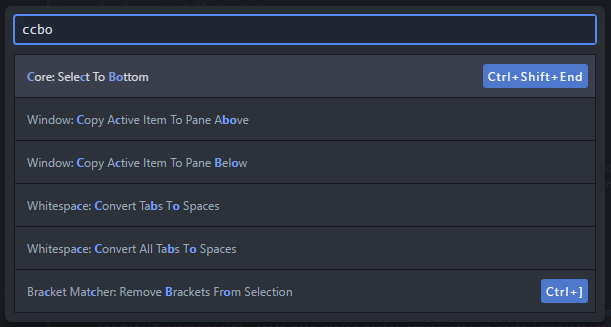
\includegraphics[scale = 0.7]{paleta}
		\caption{Paleta de Comandos do Atom no Windows.}
	\end{figure}

	A busca na Paleta de Comandos é extremamente eficiente, uma vez que faz uso de uma expressão regular baseada unicamente na ordem dos caracteres inseridos. Além de encontrar os comandos, o menu da paleta também exibe os atalhos de tecla associados a eles. Mais da Paleta de Comandos será explorada durante este artigo.

	\subsubsection{Configurações e Preferências}
	No Atom, as Configurações e Preferências podem ser modificadas no Painel (costumeiramente referenciado na literatura como \textit{View}) de Configurações. As opções variam entre a troca de tema, quebras de linha, tamanho da tabulação, velocidade do \textit{scroll} e gerenciamento de pacotes (\textit{Packages}, a ser tratado na Seção \ref{sec:packages}).

	Cabe salientar que essas informações são mantidas na pasta \textit{.atom}.

	O acesso ao Painel de Configurações do Atom pode se dar de diferentes maneiras:
	\begin{itemize}
		\item No menu superior, \verb|File > Settings|
		\item Na Paleta de Comandos, \verb|settings-view:open|
		\item Pelo atalho de teclas padrão \verb|Ctrl + ,|
	\end{itemize}

	No Painel de Configurações, existem outros paineis anexados, conforme se nota no menu lateral. As opções permitem visualizar categorias específicas das configurações, o que facilita ao usuário encontrar a alteração que deseja realizar.

	Neste menu também é possível encontrar a opção para alterar os temas do Atom. Por padrão, o Atom possui quatro diferentes temas de Interface Gráfica, claras e escuras, bem como oito temas diferentes para sintaxe. Os temas de Interface Gráfica controlam elementos como as abas e menus, enquanto os temas de Sintaxe modificam o destaque de sintaxe (\textit{syntax highlighting}). Além disso, há a possibilidade do usuário baixar um tema pronto do repositório do Atom em \href{https://atom.io}{https://atom.io}, customizar um tema já existente (mais informações em \href{http://flight-manual.atom.io/using-atom/sections/basic-customization/}{http://flight-manual.atom.io/using-atom/sections/basic-customization/}) ou criar seu próprio tema (mais informações em \href{http://flight-manual.atom.io/hacking-atom/sections/creating-a-theme/}{http://flight-manual.atom.io/hacking-atom/sections/creating-a-theme/}).

	Outro recurso interessante que pode ser encontrado neste Painel é a quebra de linha automática. Isso é particularmente útil ao fazer do Atom um editor de documentos (principalmente em \LaTeX). O recurso está disponível neste mesmo Painel de Configurações, permitindo inclusive substituir espaços por tabulações e vice-versa.

	\subsubsection{Pastas de Projeto}
	O Atom possui uma estrutura chamada de Árvore de Visualização (\textit{Tree View}), por padrão anexada ao menu lateral esquerdo, onde o usuário pode visualizar toda a hierarquia de diretórios e arquivos que está manipulando, o que permite navegar com facilidade entre os mesmos para que sejam editados com um único clique. Pode-se alternar a exibição da Árvore com \verb|Ctrl + \| e focar através de \verb|Alt + \|. Quando a Árvore possui foco, pode-se pressionar \verb|A| para adicionar um arquivo, \verb|M| para movê-lo e \verb|Delete| para deletá-lo.

	Para adicionar uma Pasta de Projeto (\textit{Project Folder}) e, desse modo, constar na Árvore de Visualização, pode-se utilizar o menu superior em \verb|File > Add Project Folder| ou usar o atalho padrão \verb|Ctrl + Shift + A| e navegar até a pasta desejada.

	\subsubsection{Packages}\label{sec:packages}


	\section{Hackeando o Atom}

	\subsection{Hackeando o Núcleo do Atom} \label{sec:hackingcore}


	\section{Conclusão e Análise}
	Dentre as análises

	\bibliographystyle{sbc}
	\bibliography{references}

\end{document}
